\documentclass[11pt,a4paper]{article}
\usepackage{graphicx}
\usepackage{hyperref}

\title{Fundamentals of Machine Learning \\ Exercise Sheet 8: \\ Mini-Research-Project Ideas}
\author{Max Simon, Debora Fieberg}

\begin{document}
	\maketitle
	
	\centerline{\large{\textbf{Project 1: Plane Trajectories}}}
	\bigskip
	Our first project idea is to use a machine learning ansatz for more accurate predictions of plane trajectories.	
	In specific, we are interested in a regression analysis of the Cruise Climb Rate (FL 100 to FL 285, FL = flight level) using data of the Initial Climb Rate of the airplane. A successful prediction would be extremely useful for Controller Assistance Tools (CATO) of the Deutsche Flugsicherung (DFS), which are currently being developed to warn and assist air traffic controllers at centers and towers. Momentary calculations concerning the climb rate are rather inaccurate so that a big buffer is needed for safety ($\pm 1500$ ft/min for rates around $\frac{50}{6000}$ ft/min.). Better predictions could reduce this buffer leading to less false alarms of conflicts, less maneuvers to be made and ultimately more accurate commands given to the pilots. \\
	 
	The project is an actual research question of the research and development team of the DFS (Deutsche Flugischerung). They would provide us with a sufficiently big data set (up to 30 days of aviation data) including recording time, track number, aircraft type, roll angle, selected altitude, track angle, ground speed, true airspeed, magnetic heading, indicated airspeed, Mach, altitude rate, inertial vertical velocity and much more. Part of a typical dataset of an airbus can be seen in Figure 1. \\
	
	\begin{figure} 
		\centering
		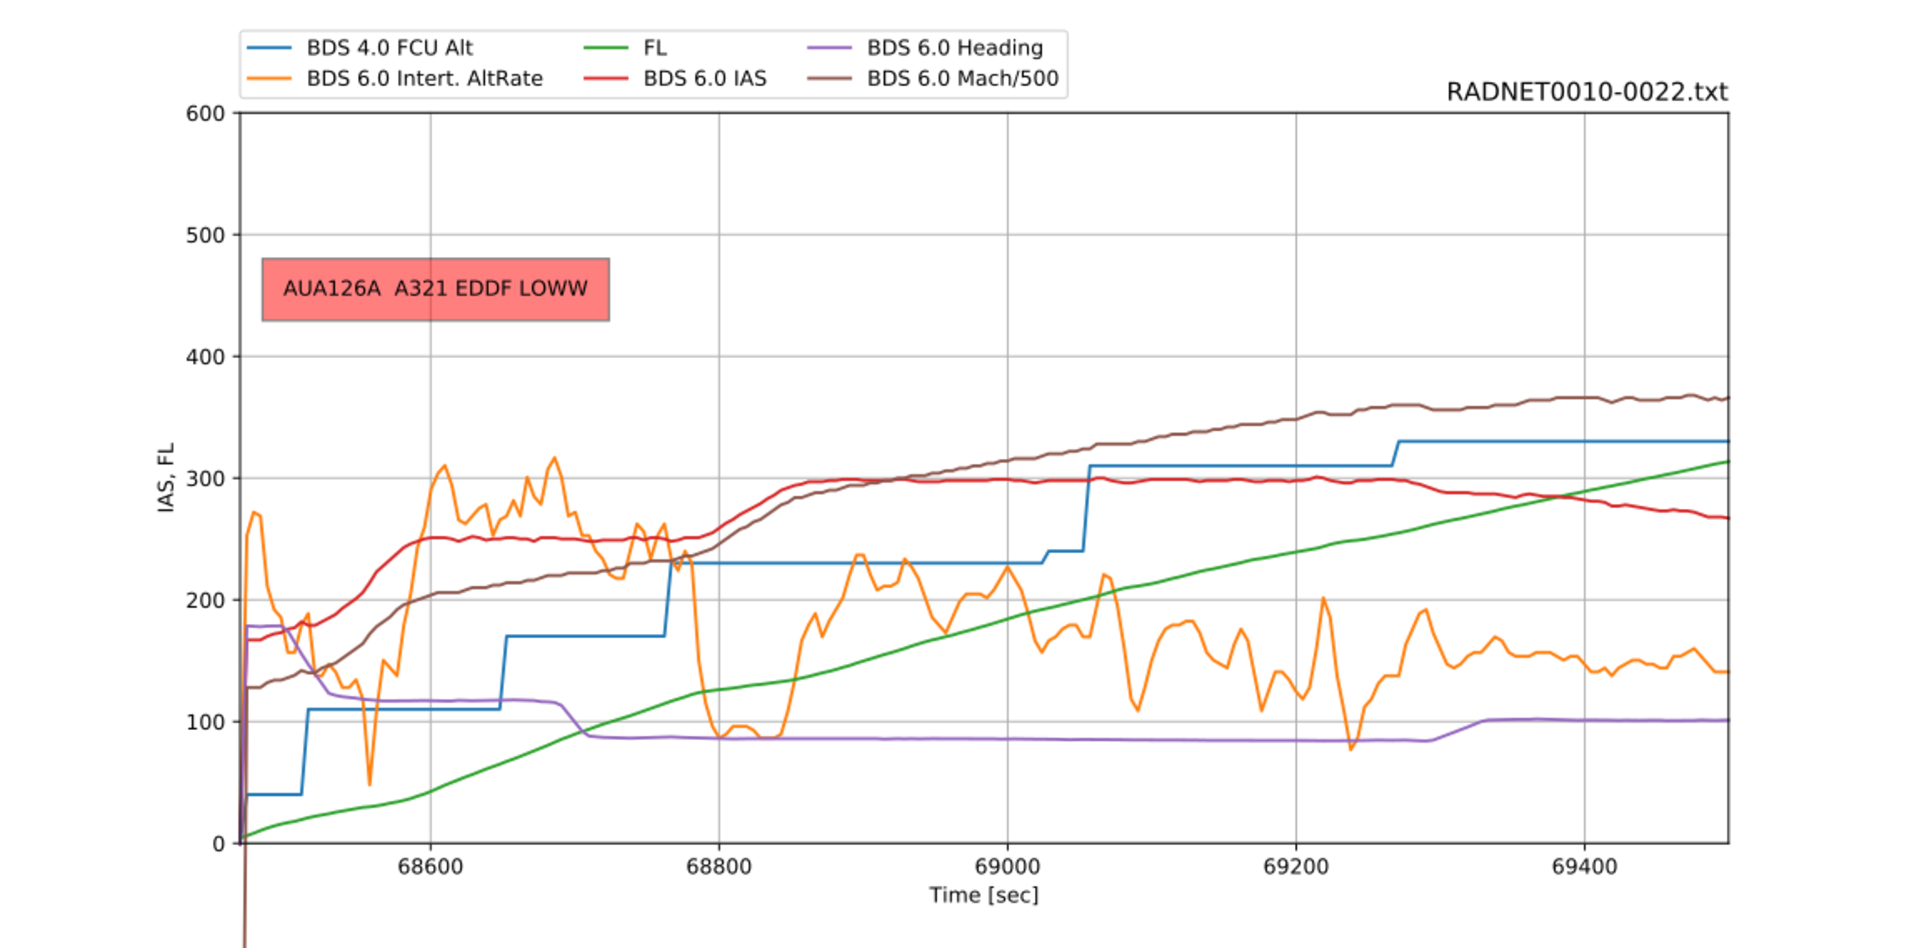
\includegraphics[width=1.0\textwidth]{AUA126A.pdf}
		\caption{Visualization of DFS Data}	
	\end{figure}
	
	Afterwards, there might even be a possibility to test our results in a full flight simulator. Instead of considering the Rate of Climb (ROC) it might also be useful to directly investigate the flight level, which ideally should be the integral of the ROC. Those two measures yield different measures close to ground level so that we need to clarify whether the dependence is yet influential for the data after FL 100.\\
	\\
	With the given data we will perform a non-linear regression to predict the climb rate. To this end, we will use support vector regression or a multi-layer neural network. The exact design and hyperparameter tuning will be part of the evaluation.
	
	\bigskip
	\centerline{\large{\textbf{Project 2: Movies}}}
	\bigskip
	
	In this project we want to investigate a dataset on movies which can be found on Kaggle\footnote{\url{https://www.kaggle.com/stephanerappeneau/350-000-movies-from-themoviedborg}, 07.01.18, 15:00}. The dataset contains about 329000 entries and provides information on the film (like the title, genre and release date) as well as information on the success (popularity and user votes).\\
	\\
	We will use this dataset to approach the question, how the film title might influence the success of the film with respect to its genre and release date.\\
	To this end we will process the film titles for different subsets of the dataset and correlate them with the success indicators of the film. For the textprocessing we will use common techniques like stemming or lematizing and construct different features from it (e.g. word bags, first word of title, etc).\\
	\\
	This investigation might reveal outstanding keywords which attracts people to different movie genres and how they changed over time. Also an automatic title creation from the learned importances might be possible.
	
	%\bigskip
	%\centerline{\large{\textbf{Project 3: DB}}}
	%\bigskip
	%Raphael
	
\end{document}